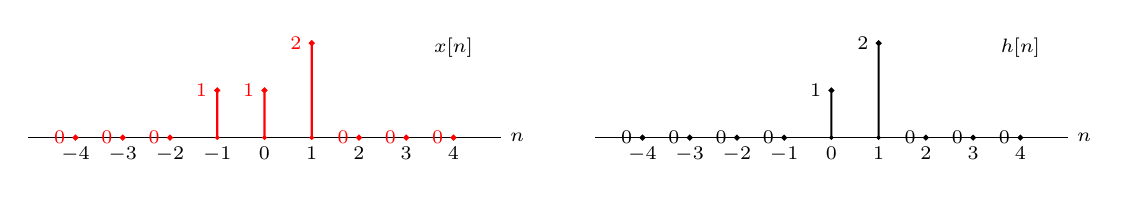
\begin{tikzpicture}[scale=0.6]

	\def\nmin{-4}
	\def\nmax{4}	
	
	\begin{scope}	
		\def\x{{0, 0, 0, 1, 1, 2, 0, 0, 0}}	

		\draw (\nmin-1, 0) -- (\nmax+1,0) node[anchor=west] {\scriptsize $n$};
		\foreach \n in {\nmin, ..., \nmax}
		{
			\node at (\n, 0) [anchor=north] {\scriptsize $\n$};
		}
		\node at (\nmax,1.5) [anchor=south] {\scriptsize $x[n]$};
		
		\foreach \n in {0,1, ...,8}
		{
			\pgfmathparse{\x[\n]}
			\edef\xn{\pgfmathresult}	
			\ifthenelse{\xn > 0}
			{
				\draw[red, thick, fill=red]  (\n + \nmin, 0) -- ++(0, \xn) circle (1pt) node[anchor=east] {\scriptsize $\xn$};
			}
			{
				\draw[red, fill=red] (\n+ \nmin,  0) circle (1pt);
			}
		}
	\end{scope}	
	
	\begin{scope}[xshift=12cm, yshift=0cm]	
		\def\h{{0, 0, 0, 0, 1, 2, 0, 0, 0}}	
		\draw (\nmin-1, 0) -- (\nmax+1,0) node[anchor=west] {\scriptsize $n$};
		\foreach \n in {\nmin, ..., \nmax}
		{
			\node at (\n, 0) [anchor=north] {\scriptsize $\n$};
		}
		\node at (\nmax,1.5) [anchor=south] {\scriptsize $h[n]$};
		
		\foreach \n in {0,1, ...,8}
		{
			\pgfmathparse{\h[\n]}
			\edef\hn{\pgfmathresult}	
			\ifthenelse{\hn > 0}
			{
				\draw[thick, fill=black]  (\n + \nmin, 0) -- ++(0, \hn) circle (1pt) node[anchor=east] {\scriptsize $\hn$};
			}
			{
				\draw[fill=black] (\n+ \nmin,  0) circle (1pt);
			}
		}
	\end{scope}		
	

\end{tikzpicture}

